% Capítulo 6 - Plan de implementación (V3: sin análisis de costo-beneficio)

\chapter{Plan de implementación}\label{cap:implementacion}

Los capítulos anteriores muestran que el sistema funciona como prueba de concepto
(TRL~3). Este capítulo propone cómo podría continuarse: qué implicaría llevarlo a
operación en la Unidad Judicial de Accidentología Vial en términos de desarrollo,
equipamiento, capacitación de los usuarios, tiempos y recursos; cómo se integraría a la
rutina de trabajo de la Unidad, y con qué indicadores podría evaluarse su impacto. Da
respuesta al objetivo específico OE6.

El plan se organiza según los niveles de madurez de ISO~16290 (\cref{sec:iso16290}) y
toma como punto de partida las condiciones de salida definidas en la gestión de riesgos
(R2, R4 y R7) y los requerimientos pendientes de la \cref{tab:requerimientos}. Su
horizonte es TRL~7, es decir, un prototipo funcionando en el entorno operativo real; la
calificación formal y el uso generalizado (TRL~8 y~9) quedan para una etapa posterior.

% ------------------------------------------------------------
\section{Etapas del plan}\label{sec:impl-etapas}

La \cref{tab:impl-etapas} describe las siete etapas propuestas, sus entregables y el
criterio que debe cumplirse para darlas por terminadas. La ejecución mantendría la
metodología híbrida del proyecto, corrigiendo la debilidad identificada en la
\cref{ssec:balance-metodologia}: sprints de dos semanas con una revisión con el
Ministerio Público Fiscal al cierre de cada uno, y un tablero Kanban para la gestión
interna de las tareas.

La etapa central del plan es la \emph{validación en modo sombra}. En esa modalidad el
sistema opera en paralelo con el procedimiento vigente, con datos reales y en tiempo
real, pero sus alertas no se comunican a quienes toman las decisiones: solo se
registran, para compararlas después con los siniestros efectivamente ocurridos. Así
puede medirse el desempeño del sistema en condiciones reales sin exponer a la Unidad
Judicial a las consecuencias de sus errores. Como el procedimiento vigente no se
modifica durante esa etapa, el período sirve además para relevar la situación actual
contra la que se evaluará el impacto (\cref{sec:impl-impacto}).

{\setstretch{1.0}\small
\begin{longtable}{@{}>{\raggedright\arraybackslash}p{0.17\textwidth}
                    >{\raggedright\arraybackslash}p{0.38\textwidth}
                    >{\raggedright\arraybackslash}p{0.22\textwidth}
                    >{\raggedright\arraybackslash}p{0.16\textwidth}@{}}
\caption{Etapas del plan de implementación}
\label{tab:impl-etapas} \\
\toprule
\textbf{Etapa (semanas)} & \textbf{Actividades principales} & \textbf{Entregable} & \textbf{Criterio de salida} \\
\midrule
\endfirsthead
\multicolumn{4}{@{}l}{\footnotesize\textit{Tabla \ref{tab:impl-etapas} (continuación)}} \\
\toprule
\textbf{Etapa (semanas)} & \textbf{Actividades principales} & \textbf{Entregable} & \textbf{Criterio de salida} \\
\midrule
\endhead
\bottomrule
\endfoot
E0. Formalización y lanzamiento (1--2)
  & Acuerdo de alcance con el MPF dentro del convenio vigente; designación de
    referentes funcional y de datos; definición de la cadencia de revisión.
  & Acta de inicio y plan de trabajo aprobado.
  & Referentes designados. \\
E1. Condiciones de salida de TRL~3 (2--7)
  & Medición de la latencia entre el siniestro y su carga (R2); verificación de
    unicidad por cuasi-identificadores (R4); diseño del procedimiento de validación
    humana de las alertas (R7); acuerdo con el MPF sobre los registros necesarios para
    medir los indicadores de impacto.
  & Informe de latencia, informe de reidentificación, procedimiento de validación y
    fuentes de los indicadores.
  & R2, R4 y R7 tratados. \\
E2. Integración en laboratorio, TRL~4 (7--15)
  & Ingesta automatizada desde la base del MPF; servicio de predicción en el CCAD;
    capa de decisión de tres niveles; tablero de alertas en el sistema de gestión de
    siniestros; registro de alertas y decisiones (RF7).
  & Sistema integrado en entorno de laboratorio.
  & Componentes validados en conjunto (TRL~4). \\
E3. Validación en modo sombra, TRL~5--6 (16--27)
  & Operación en paralelo con datos reales, sin intervenir en las decisiones;
    comparación semanal entre alertas y siniestros; recalibración del umbral con el
    MPF en términos de alertas y omisiones por semana; reentrenamiento con los datos
    2025--2026; relevamiento de la línea base de los indicadores de impacto.
  & Informe de desempeño en entorno relevante, umbral acordado y línea base de los
    indicadores.
  & Desempeño estable y aceptado por el MPF (TRL~6). \\
E4. Capacitación y gestión del cambio (23--29)
  & Manual de usuario; dos talleres por turno; prueba de usabilidad con cuestionario
    SUS; definición, junto con el MPF, de las acciones asociadas a cada nivel de
    alerta.
  & Usuarios capacitados y acciones por nivel acordadas.
  & Usabilidad aceptable según SUS. \\
E5. Piloto operativo, TRL~7 (29--39)
  & Uso real en la Unidad Judicial con validación humana registrada; seguimiento de
    la disponibilidad del servicio; medición de los indicadores de impacto
    (\cref{tab:impl-indicadores}).
  & Registro del piloto e indicadores medidos.
  & Prototipo operando en entorno real (TRL~7). \\
E6. Evaluación y transferencia (39--42)
  & Nueva evaluación de impacto (ISO/IEC~42001, 6.1.4); comparación de los
    indicadores con la línea base; plan de mantenimiento y reentrenamiento;
    documentación y transferencia (R11).
  & Informe final de impacto y plan de operación.
  & Decisión de continuidad del MPF. \\
\end{longtable}
}
\notaflot{\fuentepropia. Las semanas se cuentan desde el inicio
del plan; las etapas E3 y E4 se superponen parcialmente.}

% ------------------------------------------------------------
\section{Cronograma}\label{sec:impl-cronograma}

La \cref{fig:gantt-implementacion} presenta el cronograma del plan, de 42 semanas (unos
diez meses). El camino crítico pasa por las condiciones de salida de TRL~3, la
integración en laboratorio, la validación en modo sombra y el piloto operativo, dado que
cada una de esas etapas requiere los resultados de la anterior. La capacitación se ubica
al final de la validación en modo sombra para que los usuarios se formen con el sistema
ya calibrado y lleguen al piloto sin una brecha de tiempo que diluya lo aprendido.

\begin{figure}[htbp]
\centering
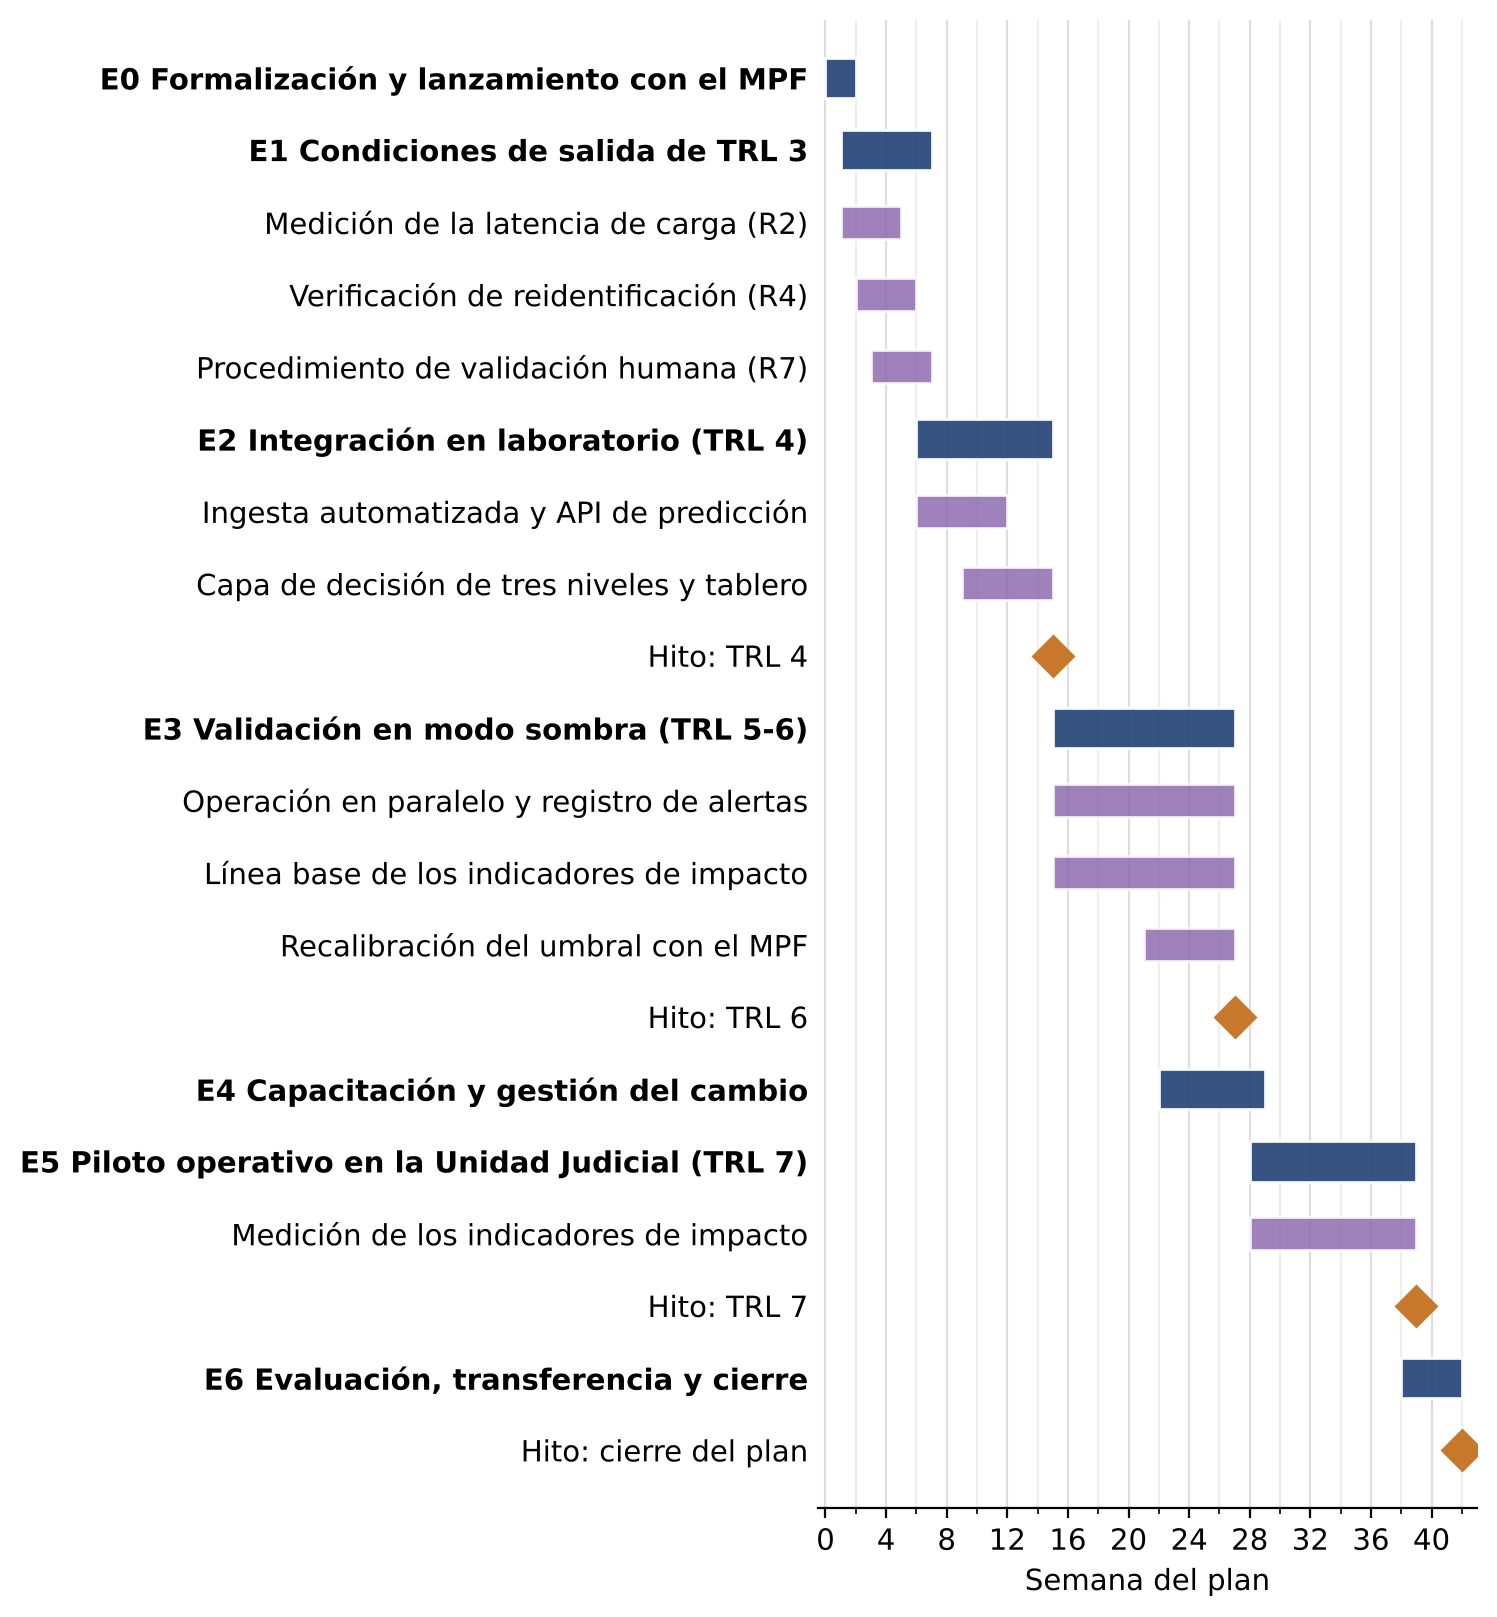
\includegraphics[width=\linewidth]{imagenes/gantt_implementacion.png}
\caption{Cronograma del plan de implementación}
\label{fig:gantt-implementacion}
\notaflot{\fuentepropia. Las barras oscuras representan etapas,
las claras tareas y los rombos hitos de madurez tecnológica.}
\end{figure}

% ------------------------------------------------------------
\section{Desarrollo, equipamiento y capacitación}\label{sec:impl-recursos}

\paragraph{Desarrollo.} El desarrollo pendiente se concentra en la etapa E2 y
corresponde a los requerimientos de la \cref{tab:requerimientos} que no se implementaron
en la prueba de concepto: la ingesta automatizada de los datos, el servicio de
predicción, la escala de tres colores, el registro de las alertas y de las decisiones
humanas, el control de acceso por roles y la disponibilidad del servicio. El modelo no
requiere cambios de arquitectura, pero sí un reentrenamiento con los datos de 2025 y
2026 que LIDeSIA está incorporando.

\paragraph{Equipamiento.} No se prevé la compra de equipamiento. El servicio y los
entrenamientos se alojan en la infraestructura del CCAD, a la que LIDeSIA accede en el
marco de sus proyectos, y los usuarios acceden al tablero desde los puestos de trabajo
existentes mediante un navegador web. Todo el software es de código abierto (RNF2). El
único requerimiento adicional es un esquema de contingencia para el servidor (R8), que
puede resolverse con una segunda instancia dentro del mismo CCAD.

\paragraph{Capacitación.} Los usuarios son profesionales del derecho sin formación
estadística, por lo que la capacitación debe centrarse en cómo leer una alerta y qué
hacer con ella, y no en el modelo. Se proponen dos talleres de tres horas por turno de
trabajo: el primero sobre la lectura de la escala de colores, la incertidumbre del
pronóstico y los errores esperables (alrededor de cinco falsas alarmas y dos o tres
omisiones por semana, según la \cref{tab:res-operativa}); el segundo, práctico, sobre las
acciones asociadas a cada nivel, el procedimiento de validación humana y el registro de
las decisiones. La capacitación se complementa con un manual breve y con la aplicación del
cuestionario SUS (\textit{System Usability Scale}), el mismo instrumento empleado en las
pruebas de usabilidad del sistema de gestión de siniestros. El SUS es un cuestionario
estandarizado de diez afirmaciones que el usuario valora en una escala de cinco puntos y
que se resume en un puntaje de 0 a 100 \parencite{brooke1996}. Un puntaje de 68 o más
se considera aceptable, por ubicarse por encima del promedio de referencia del
instrumento \parencite{sauro2011}.

\paragraph{Recursos humanos.} La \cref{tab:impl-equipo} reúne los perfiles necesarios
para la implementación y las tareas de cada uno. El equipo técnico se compone de tres
perfiles de LIDeSIA; del lado del Ministerio Público Fiscal, la participación de dos
referentes es indispensable para validar los datos, el umbral y las acciones asociadas a
cada nivel de alerta.

\begin{table}[htbp]
\centering
\caption{Perfiles necesarios para la implementación y sus tareas}
\label{tab:impl-equipo}
\begin{tabularx}{\linewidth}{@{}>{\raggedright\arraybackslash}p{0.30\textwidth}
                                >{\raggedright\arraybackslash}X@{}}
\toprule
\textbf{Perfil} & \textbf{Tareas principales} \\
\midrule
\textit{Product Owner} (LIDeSIA)
  & Coordinación con el MPF, gestión del plan, definición de las acciones por nivel de
    alerta, capacitación y seguimiento de los indicadores de impacto. \\
Científico de datos (LIDeSIA)
  & Reentrenamiento del modelo, calibración del umbral y seguimiento del desempeño. \\
Ingeniero de datos y desarrollo (LIDeSIA)
  & Ingesta automatizada, servicio de predicción, tablero de alertas y registro de
    decisiones. \\
\midrule
Referente funcional de la Unidad Judicial (MPF)
  & Validación del umbral y de las acciones por nivel de alerta; vínculo con los
    usuarios. \\
Referente de datos (MPF)
  & Acceso a los datos, medición de la latencia de carga y anonimización. \\
Usuarios de la Unidad Judicial (MPF)
  & Participación en los talleres de capacitación y en la prueba de usabilidad. \\
\bottomrule
\end{tabularx}
\notaflot{\fuentepropia.}
\end{table}

Una vez concluido el plan, la operación requeriría un científico de datos a tiempo
parcial para el seguimiento del desempeño y los reentrenamientos periódicos, y la
participación del referente de datos del MPF para sostener la calidad y la oportunidad de
la carga.

% ------------------------------------------------------------
\section{Integración en la operación de la Unidad Judicial}\label{sec:impl-operacion}

El sistema no reemplaza el procedimiento de la Unidad Judicial: le agrega, antes de cada
bloque de seis horas, una estimación del riesgo esperado que el responsable de turno usa
para organizar la guardia. En operación, el flujo de la \cref{fig:flujograma} se
traduciría en el siguiente ciclo, que se repite cuatro veces por día:

\begin{enumerate}[leftmargin=*,itemsep=2pt]
  \item Al cierre de cada bloque, la ingesta toma los siniestros cargados hasta ese
        momento en el sistema de gestión y actualiza la serie.
  \item El modelo estima el riesgo del bloque siguiente y la capa de decisión lo traduce
        en un nivel de alerta: verde, amarillo o rojo.
  \item La alerta se publica en el tablero antes del inicio del bloque, junto con las
        variables que más influyeron en la estimación.
  \item El responsable de turno valida la alerta y decide qué acción tomar, según las
        acciones acordadas para cada nivel en la etapa E4; puede apartarse de ellas
        indicando el motivo.
  \item La alerta y la decisión quedan registradas (RF7).
  \item Semanalmente, el equipo técnico compara las alertas con los siniestros ocurridos
        y controla el desempeño del modelo.
\end{enumerate}

% ------------------------------------------------------------
\section{El costo de los siniestros viales como contexto}\label{sec:impl-contexto}

Los siniestros viales tienen un costo económico considerable. Un estudio del Banco
Mundial financiado por Bloomberg Philanthropies estima que una reducción del
\qty{10}{\percent} en las muertes por siniestros viales eleva el producto bruto interno per
cápita en un \qty{3.6}{\percent} en un horizonte de 24 años
\parencite{bloomberg2018,worldbank2017}, y el Global Road Safety Facility estima que los
siniestros cuestan a las economías de ingresos bajos y medios entre el 2 y el
\qty{6}{\percent} de su producto bruto interno cada año \parencite{grsf2025}. Para la
Argentina, la Agencia Nacional de Seguridad Vial estimó el costo social de la
siniestralidad de 2017 en el \qty{1.7}{\percent} del producto bruto interno, con costos
unitarios de \$30.551.793 por fallecido, \$284.111 por herido grave y \$3375 por herido
leve \parencite{ansv2019}. Esos costos incluyen la atención médica, la pérdida de
productividad, los costos humanos, los daños materiales y los costos administrativos,
entre ellos los policiales y judiciales.

En cuanto al costo sanitario, un estudio realizado en un hospital público de referencia
de Tucumán estimó un costo directo promedio de hospitalización de \$39.950 por paciente
lesionado en el tránsito en 2017, equivalentes a USD~2350 \parencite{herrerabruno2019}.
No se encontraron estimaciones publicadas para el Hospital Municipal de Urgencias de
Córdoba, principal receptor de los lesionados de la ciudad, por lo que se adoptan las
referencias nacionales.

La \cref{tab:impl-costo-social} aplica los costos unitarios de la ANSV a los siniestros
de la base de este trabajo. Como la base registra siniestros por su carátula y no
personas, y un siniestro puede tener más de una víctima, el resultado es una cota
inferior.

\begin{table}[htbp]
\centering
\caption{Costo social anual estimado de los siniestros de la base}
\label{tab:impl-costo-social}
\begin{tabularx}{\linewidth}{@{}>{\raggedright\arraybackslash}X
                                >{\raggedleft\arraybackslash}p{0.15\textwidth}
                                >{\raggedleft\arraybackslash}p{0.19\textwidth}
                                >{\raggedleft\arraybackslash}p{0.19\textwidth}@{}}
\toprule
\textbf{Carátula} & \textbf{Siniestros por año} & \textbf{Costo unitario (USD 2017)}
  & \textbf{Costo anual (M USD 2017)} \\
\midrule
Homicidio culposo              & 46   & 1.797.164 & 82,7 \\
Lesiones graves o gravísimas   & 401  & 16.712    & 6,7 \\
Lesiones leves                 & 1546 & 199       & 0,3 \\
\midrule
Total                          & 1993 &           & 89,7 \\
\bottomrule
\end{tabularx}
\notaflot{Elaboración propia a partir de los siniestros clasificados
de la figura 4.7 (dos años de registro) y de los costos unitarios de
\textcite{ansv2019}, convertidos a dólares con el tipo de cambio de 2017 implícito en
\textcite{herrerabruno2019} (\$17 por dólar). Los valores no están actualizados por
inflación, por lo que subestiman el costo actual.}
\end{table}

El costo social de los siniestros con intervención judicial en la ciudad de Córdoba se
ubica en el orden de los USD~90 millones anuales, aun con valores de 2017. Estas cifras
dan la escala del problema sobre el que interviene el Ministerio Público Fiscal y
muestran el peso de la respuesta institucional que motiva este trabajo.

Sin embargo, el impacto económico del sistema no puede cuantificarse a partir de ellas.
El producto no está orientado a reducir la cantidad ni la gravedad de los siniestros,
sino a anticipar la demanda que generan sobre los recursos de la Unidad Judicial: actúa
sobre la organización de la respuesta institucional y no sobre la ocurrencia de los
hechos. Atribuirle una fracción de esos costos supondría un vínculo causal que el sistema
no tiene. Tampoco se dispone de información sobre dotaciones ni remuneraciones del
Ministerio Público Fiscal que permita valorar en dinero los cambios en el uso de sus
recursos. Por estas razones no se realiza un análisis de costo-beneficio, y el impacto de
la implementación se evalúa mediante los indicadores operativos y de calidad de la
decisión que se presentan a continuación.

% ------------------------------------------------------------
\section{Evaluación del impacto de la implementación}\label{sec:impl-impacto}

El impacto se evalúa comparando el funcionamiento de la Unidad Judicial sin el sistema y
con él. La validación en modo sombra cumple un doble papel: mientras el sistema opera sin
intervenir, el procedimiento vigente sigue intacto, por lo que los indicadores relevados
en ese período constituyen la línea base. Durante el piloto se miden los mismos
indicadores con el sistema en uso. La diferencia entre ambos períodos, interpretada junto
con la estacionalidad propia de la siniestralidad, es la evidencia de impacto. La
\cref{tab:impl-indicadores} reúne los indicadores propuestos, agrupados en seis
dimensiones.

{\setstretch{1.0}\small
\begin{longtable}{@{}>{\raggedright\arraybackslash}p{0.16\textwidth}
                    >{\raggedright\arraybackslash}p{0.33\textwidth}
                    >{\raggedright\arraybackslash}p{0.24\textwidth}
                    >{\raggedright\arraybackslash}p{0.19\textwidth}@{}}
\caption{Indicadores para evaluar el impacto de la implementación}
\label{tab:impl-indicadores} \\
\toprule
\textbf{Dimensión} & \textbf{Indicador} & \textbf{Fuente y etapa} & \textbf{Referencia} \\
\midrule
\endfirsthead
\multicolumn{4}{@{}l}{\footnotesize\textit{Tabla \ref{tab:impl-indicadores} (continuación)}} \\
\toprule
\textbf{Dimensión} & \textbf{Indicador} & \textbf{Fuente y etapa} & \textbf{Referencia} \\
\midrule
\endhead
\bottomrule
\endfoot
Desempeño en operación real
  & Sensibilidad en clase crítica y en clase normal; falsas alarmas y omisiones por
    semana, frente a la regla de alerta permanente.
  & Comparación semanal entre alertas y siniestros (E3 y E5).
  & No inferior a la prueba de concepto (\cref{tab:res-baseline-referencia}). \\
Uso de los recursos
  & Horas-persona de guardia asignadas en bloques verdes frente a rojos; proporción de
    turnos organizados según el nivel de alerta.
  & Registro de dotaciones por turno (E3 y E5).
  & Mayor dotación en los bloques de mayor riesgo que en la línea base. \\
Oportunidad de la respuesta
  & Tiempo entre la toma de conocimiento del siniestro y la intervención pericial o de
    la Policía Judicial, según el nivel de alerta del bloque.
  & Sistema de gestión de siniestros (E3 y E5).
  & Igual o menor que en la línea base. \\
Trazabilidad de la decisión
  & Proporción de alertas con decisión registrada; proporción de decisiones que se
    apartan de la sugerencia y sus motivos.
  & Registro de alertas y decisiones, RF7 (E5).
  & Todas las alertas con decisión registrada. \\
Adopción y confianza
  & Puntaje SUS; frecuencia de consulta del tablero; percepción de utilidad; alertas
    desestimadas como señal de fatiga.
  & Cuestionario, registros de acceso y entrevistas (E4 y E5).
  & SUS de 68 o más (usabilidad aceptable). \\
Calidad del proceso de datos
  & Latencia entre el siniestro y su carga; proporción de bloques con datos completos
    al momento de predecir.
  & Fechas del hecho y de la carga (E1, E3 y E5).
  & Menor latencia que la medida en E1. \\
\end{longtable}
}
\notaflot{\fuentepropia. Las referencias son orientativas y se
acuerdan con el Ministerio Público Fiscal al cierre de la etapa E3.}

Estos indicadores se miden con registros que el propio organismo genera, sin supuestos
externos, y se vinculan directamente con la necesidad que dio origen al trabajo:
dimensionar la respuesta según el riesgo esperado y no como si todos los bloques fueran
críticos. Son, además, la información que el Ministerio Público Fiscal necesitaría para
decidir la continuidad del sistema al final de la etapa E6. La dimensión de calidad del
proceso de datos merece una mención aparte: como el techo del desempeño lo fija la carga
de los siniestros (\cref{cap:conclusiones}), una mejora en la latencia es a la vez un
impacto de la implementación y una condición para que las demás dimensiones mejoren.

La implementación tiene también impactos que no se expresan en un indicador. La
asignación de recursos pasaría a apoyarse en un criterio explícito y trazable, en lugar
de una sobreasignación permanente sin fundamento cuantitativo. La base de siniestros
curada y transformada en serie temporal queda como un activo del organismo para otros
análisis. Y el procedimiento completo, desde la carga hasta la decisión registrada, puede
replicarse en otras unidades judiciales que atienden hechos con demanda variable,
siempre con una nueva evaluación de impacto (R10).

% ------------------------------------------------------------
\section{Síntesis}\label{sec:impl-sintesis}

La implementación requiere unos diez meses, un equipo de tres perfiles técnicos de
LIDeSIA y la participación de dos referentes del Ministerio
Público Fiscal, sin compra de equipamiento ni licencias. El sistema se integraría a la
rutina de la Unidad Judicial como una alerta por bloque de seis horas, validada por el
responsable de turno y asociada a acciones por nivel que se acuerdan con el Ministerio
Público Fiscal.

Como el producto no actúa sobre la ocurrencia de los siniestros, su impacto no se mide
en términos económicos, sino con indicadores de desempeño, uso de los recursos,
oportunidad de la respuesta, trazabilidad, adopción y calidad de los datos, relevados
primero en modo sombra y luego en el piloto. La principal incertidumbre es la
disponibilidad de los registros del Ministerio Público Fiscal necesarios para construir
la línea base, que el plan prevé acordar desde la etapa E1.
